\documentclass[tikz,border=8pt]{standalone}
% Shared look for every TikZ diagram. Load with \input{../../tools/tikz-style.tex}
\usepackage[T1]{fontenc}
\usepackage{lmodern}
\renewcommand{\sfdefault}{lmr}  % diagrams use the same serif as the text
\usetikzlibrary{arrows.meta, positioning, shapes.geometric, calc, fit, backgrounds}
\definecolor{cblue}{HTML}{4C78A8}
\definecolor{corange}{HTML}{F58518}
\definecolor{cgreen}{HTML}{54A24B}
\definecolor{cred}{HTML}{E45756}
\definecolor{cpurple}{HTML}{B279A2}
\definecolor{cgrey}{HTML}{6B6B6B}
\tikzset{
  every picture/.style={font=\sffamily, line width=1.2pt},
  box/.style={draw=#1, fill=#1!12, rounded corners=4pt, align=center, inner sep=7pt, minimum height=1.1cm},
  box/.default=cgrey,
  arrow/.style={-{Stealth[length=3mm]}, draw=cgrey, line width=1.4pt},
  title/.style={font=\sffamily\bfseries\Large},
  note/.style={font=\sffamily\small, text=cgrey, align=center},
}
\AtBeginDocument{\hyphenpenalty=10000 \exhyphenpenalty=10000}

\begin{document}
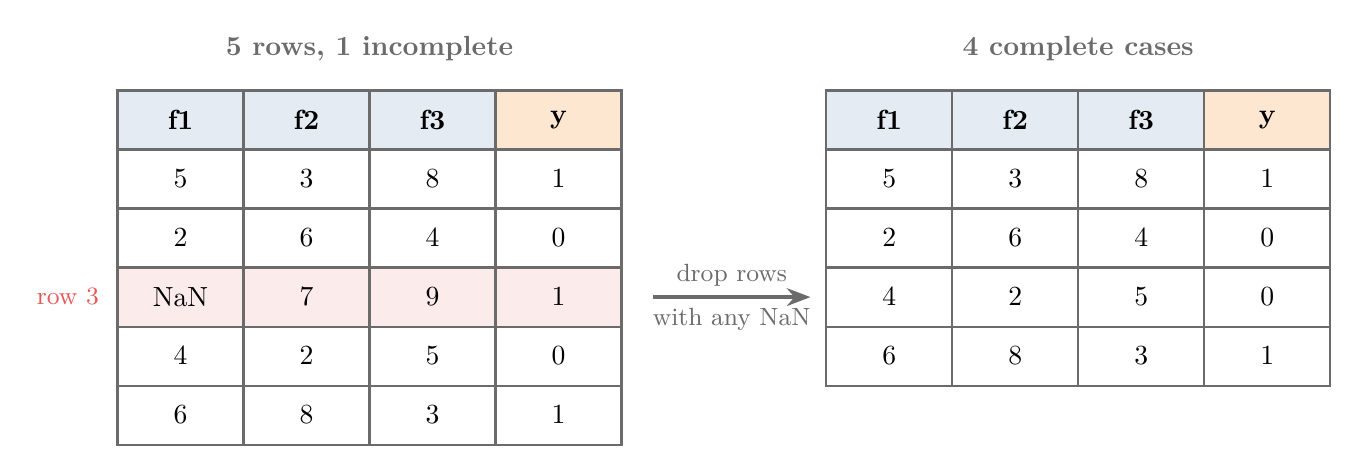
\begin{tikzpicture}[cell/.style={draw=cgrey, line width=0.8pt, minimum width=1.6cm, minimum height=0.75cm, font=\sffamily}]
  % before: 5 rows, row 3 has a missing f1
  \fill[cred!12] (0.8,-2.625) rectangle (7.2,-1.875);
  \foreach \x in {0,9} {
    \foreach \h [count=\j] in {f1,f2,f3} \node[cell, fill=cblue!15, font=\sffamily\bfseries] at (1.6*\j+\x,0) {\h};
    \node[cell, fill=corange!20, font=\sffamily\bfseries] at (6.4+\x,0) {y};
  }
  \foreach \r [count=\i] in {{5,3,8,1},{2,6,4,0},{NaN,7,9,1},{4,2,5,0},{6,8,3,1}}
    \foreach \v [count=\j] in \r \node[cell] at (1.6*\j,-0.75*\i) {\v};
  % after: row 3 removed
  \foreach \r [count=\i] in {{5,3,8,1},{2,6,4,0},{4,2,5,0},{6,8,3,1}}
    \foreach \v [count=\j] in \r \node[cell] at (1.6*\j+9,-0.75*\i) {\v};
  \node[note, anchor=east, text=cred] at (0.7,-2.25) {row 3};
  \draw[arrow] (7.6,-2.25) -- node[above, note]{drop rows} node[below, note]{with any NaN} (9.6,-2.25);
  \node[note, font=\sffamily\bfseries] at (4,0.9) {5 rows, 1 incomplete};
  \node[note, font=\sffamily\bfseries] at (13,0.9) {4 complete cases};
\end{tikzpicture}
\end{document}
